\documentclass[conference,10pt]{IEEEtran}

\usepackage[T1]{fontenc}
\usepackage[utf8]{inputenc}
\usepackage[spanish,es-noindentfirst]{babel}
\usepackage{microtype}
\usepackage{graphicx}
\usepackage{booktabs}
\usepackage{siunitx}
\usepackage{subcaption}
\usepackage{xcolor}
\usepackage{amsmath}
\usepackage[hidelinks]{hyperref}
\usepackage[capitalise,noabbrev]{cleveref}
% Spanish names for cross-references (cleveref defaults to English).
\crefname{figure}{figura}{figuras}\Crefname{figure}{Figura}{Figuras}
\crefname{table}{cuadro}{cuadros}\Crefname{table}{Cuadro}{Cuadros}
\crefname{section}{secci\'on}{secciones}\Crefname{section}{Secci\'on}{Secciones}
\crefname{equation}{ec.}{ecs.}\Crefname{equation}{Ec.}{Ecs.}
\AtBeginDocument{%
  \renewcommand{\crefpairconjunction}{ y }%
  \renewcommand{\creflastconjunction}{ y }%
  \renewcommand{\crefrangeconjunction}{ a }}

\sisetup{round-mode=places,round-precision=2,detect-weight=true}
\graphicspath{{figures/}}

\begin{document}

\title{Parameter Server vs.\ All-Reduce en entrenamiento distribuido de redes
neuronales: dise\~no y evaluaci\'on experimental en O.N.O.}

\author{\IEEEauthorblockN{Lorenzo Minervino}
\IEEEauthorblockA{Facultad de Ingenier\'ia, Universidad de Buenos Aires\\
Aprendizaje Profundo\\
Junio 2026}}

\maketitle

\begin{abstract}
El entrenamiento distribuido de redes neuronales se apoya en dos familias de
algoritmos para agregar gradientes: el \emph{Parameter Server} (PS), con servidores
centrales que concentran y actualizan los pesos, y \emph{All-Reduce} (AR), donde los
workers reducen gradientes entre s\'i sin servidor central. Presentamos O.N.O., un
sistema de entrenamiento distribuido implementado desde cero en Rust con binding
Python, en el que todos los nodos corren el mismo binario y el orquestador asigna los
roles (worker o servidor) en tiempo de ejecuci\'on. Sobre O.N.O.\ comparamos AR y PS
(este \'ultimo sincr\'onico, con barrera) en MNIST, bajo un criterio de \emph{batch
global fijo} (necesario porque en O.N.O.\ el \texttt{batch\_size} es por worker),
midiendo convergencia, throughput y escalabilidad. La evidencia observada indica que,
en este entorno homog\'eneo sobre una sola m\'aquina, All-Reduce iguala a Parameter
Server en convergencia (a batch global fijo, ambos cerca de $94.7$\,\% de accuracy a 5
nodos) y lo supera en throughput y tiempo hasta accuracy, porque el servidor central de
PS introduce un cuello de serializaci\'on. PS, en cambio, escala con pendiente m\'as
pronunciada al crecer los nodos y resulta m\'as robusto con modelos grandes. Las
conclusiones est\'an acotadas a un cl\'uster simulado sobre una \'unica m\'aquina de
ocho n\'ucleos.
\end{abstract}

\begin{IEEEkeywords}
entrenamiento distribuido, deep learning, Parameter Server, All-Reduce, Rust,
escalabilidad.
\end{IEEEkeywords}

\section{Introducci\'on}
A medida que crecen los modelos y los datos, el entrenamiento de redes neuronales se
vuelve inviable en un \'unico proceso y se distribuye sobre varios workers que
calculan gradientes en paralelo sobre particiones de los datos (SGD distribuido con
paralelismo de datos)~\cite{bennun2019demystifying}. El cuello de botella deja de ser
el c\'omputo y pasa a ser la \emph{comunicaci\'on}: c\'omo se agregan los gradientes y
c\'omo se sincronizan los pesos. Dos enfoques dominan. El \emph{Parameter Server}
mantiene los pesos en uno o m\'as servidores; los workers env\'ian gradientes y reciben
par\'ametros actualizados~\cite{li2014scaling}. \emph{All-Reduce} elimina el servidor:
los workers intercambian y promedian gradientes entre s\'i, t\'ipicamente en
anillo~\cite{gibiansky2017bringing,sergeev2018horovod}, y cada uno aplica el mismo
update.

\textbf{Pregunta de investigaci\'on.} \emph{?`Cu\'ando conviene cada enfoque, por
qu\'e, y qu\'e compromisos aparecen entre convergencia, throughput, escalabilidad y
sincronizaci\'on?} No buscamos el estado del arte en visi\'on, sino caracterizar el
\emph{sistema} de entrenamiento.

\textbf{Contribuci\'on.} (i) Describimos O.N.O., un sistema distribuido propio en
Rust donde los roles se asignan en runtime y que implementa AR y PS; (ii) aportamos una
comparaci\'on experimental honesta AR vs.\ PS sobre MNIST con un criterio de
comparaci\'on justa (\emph{batch global fijo}); y (iii) destilamos una matriz de
decisi\'on sobre cu\'ando preferir cada enfoque, acotada a las condiciones evaluadas.

\section{Fundamentos y dise\~no}

\subsection{SGD distribuido con paralelismo de datos}
Con $W$ workers, cada uno procesa un mini-batch local de tama\~no $b$ y calcula un
gradiente $g_w$. El gradiente agregado es el promedio $\bar{g}=\frac{1}{W}\sum_w g_w$,
que equivale a un paso de SGD con \emph{batch efectivo} $W\cdot b$. Promediar (y no
sumar) mantiene la magnitud del gradiente, y por ende el learning rate efectivo,
independiente de $W$. Esta distinci\'on es central: en O.N.O.\ el \texttt{batch\_size}
es \emph{por worker}, de modo que agregar workers a $b$ constante cambia el batch
efectivo (\cref{sec:fair}).

\subsection{Parameter Server}
Los servidores almacenan los pesos, posiblemente \emph{shardeados} entre varios
servidores; los workers hacen \emph{push} de gradientes y \emph{pull} de
par\'ametros~\cite{li2014scaling}. El r\'egimen de sincronizaci\'on define el
comportamiento: con \emph{barrera} todos los workers esperan a que el server aplique
el update (sincr\'onico, equivalente estad\'istico a AR); sin barrera, los workers
proceden con par\'ametros potencialmente \emph{stale}, ganando throughput a costa de
ruido (estilo Hogwild~\cite{recht2011hogwild}). En este trabajo usamos el r\'egimen
sincr\'onico (barrera con store de doble buffer), que conserva la sem\'antica de
optimizaci\'on est\'andar.

\subsection{All-Reduce}
En \emph{ring all-reduce} los $W$ workers se ordenan en anillo y ejecutan dos fases:
\emph{scatter-reduce} (cada worker termina con un fragmento del gradiente sumado) y
\emph{all-gather} (se propaga el fragmento ya reducido)~\cite{gibiansky2017bringing}.
El volumen comunicado por worker es $\approx 2\frac{W-1}{W}|g|$, independiente de $W$
salvo factor constante, lo que da buena eficiencia de ancho de banda. No hay servidor
central ni punto \'unico de contenci\'on, pero todos avanzan al ritmo del m\'as lento
(sincron\'ia estricta). O.N.O.\ promedia el gradiente reducido dividiendo por $W$.

\subsection{Arquitectura de O.N.O.}
Todas las m\'aquinas corren el mismo binario \texttt{node}. Un \texttt{orchestrator}
se conecta a todos los nodos y env\'ia una configuraci\'on de runtime que fija el rol de
cada nodo: los roles \emph{no} est\'an hardcodeados. El motor de ML, la comunicaci\'on
(protocolo y serializaci\'on) y las estrategias est\'an separados en crates de un
workspace Rust; un m\'odulo \texttt{orchestra} expone la API a Python v\'ia PyO3.
\Cref{fig:arch} resume la arquitectura y \cref{fig:concept} contrasta PS con ring
all-reduce.

\begin{figure}[t]
  \centering
  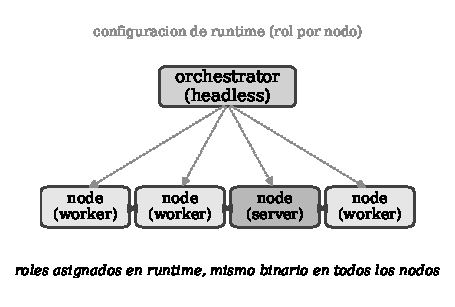
\includegraphics[width=\columnwidth]{architecture_ono.pdf}
  \caption{Arquitectura de O.N.O.: un orquestador headless asigna roles en runtime
  sobre nodos id\'enticos; seg\'un la estrategia, los nodos act\'uan como workers en
  anillo (All-Reduce) o como workers m\'as servidores (Parameter Server).}
  \label{fig:arch}
\end{figure}

\begin{figure}[t]
  \centering
  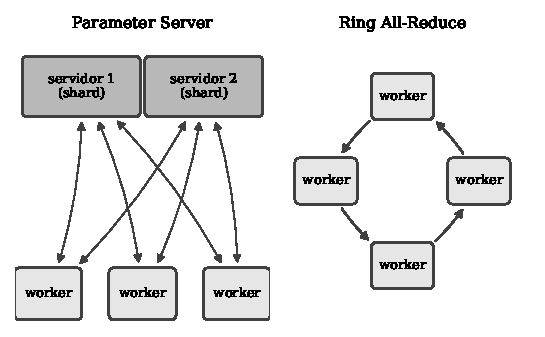
\includegraphics[width=\columnwidth]{ps_vs_ar_conceptual.pdf}
  \caption{Parameter Server (izquierda): los workers hacen push/pull contra servidores
  centrales que pueden shardear los pesos. Ring All-Reduce (derecha): los workers
  promedian gradientes entre s\'i sin servidor central.}
  \label{fig:concept}
\end{figure}

\section{Metodolog\'ia experimental}

\subsection{Datasets y modelos}
Usamos \textbf{MNIST}~\cite{lecun1998mnist} (60\,000/10\,000, 28$\times$28 en escala de grises, 10 clases,
normalizado a $[0,1]$) como benchmark base de correctitud, convergencia y
escalabilidad. \Cref{tab:datasets} resume los datasets y \cref{tab:models} las
arquitecturas. El modelo principal es \texttt{nielsen} (una CNN peque\~na con softmax
y entrop\'ia cruzada). Para aislar la presi\'on de comunicaci\'on definimos MLPs
escalables (\texttt{mlp\_small/medium/large}) cuyo objetivo no es la accuracy sino
variar el tama\~no de gradiente.

\begin{table}[t]\centering
\caption{Datasets utilizados.}\label{tab:datasets}
\footnotesize
\begin{tabular}{lrrcc}\toprule
Dataset & Train & Test & Forma & Clases\\\midrule
MNIST & 60\,000 & 10\,000 & $28\times28$ & 10\\
\bottomrule\end{tabular}
\end{table}

\begin{table}[t]\centering
\caption{Modelos y tama\~no aproximado.}\label{tab:models}
\footnotesize
\begin{tabular}{lll}\toprule
Modelo & Arquitectura & Par\'ametros\\\midrule
\texttt{nielsen} & Conv20@5--Pool--FC100--FC10 & 289\,630\\
\texttt{mlp\_small} & FC128--FC10 & 101\,770\\
\texttt{mlp\_medium} & FC512--FC512--FC10 & 669\,706\\
\texttt{mlp\_large} & FC1024--FC1024--FC10 & 1\,863\,690\\
\bottomrule\end{tabular}
\end{table}


\subsection{Estrategias y configuraciones}
Comparamos tres configuraciones: baseline single-process (PyTorch, misma receta),
All-Reduce (todos los nodos son workers) y Parameter Server (barrera con store de doble
buffer). Las topolog\'ias distribuidas se detallan en \cref{tab:configs}. Para PS con
$N$ nodos usamos $N-1$ workers y $1$ servidor. Evaluamos $N\in\{3,5\}$.

\begin{table}[t]\centering
\caption{Configuraciones distribuidas evaluadas.}\label{tab:configs}
\footnotesize
\begin{tabular}{lcccll}\toprule
Estr. & Nodos & W & S & sync/store & Batch ef.\\\midrule
AR & 3 & 3 & 0 & --/-- & 192\\
AR & 5 & 5 & 0 & --/-- & 240\\
Baseline & 1 & 1 & 0 & --/-- & 10\\
PS & 3 & 2 & 1 & barrier/blocking & 128\\
PS & 5 & 4 & 1 & barrier/blocking & 240\\
\bottomrule\end{tabular}
\end{table}


\subsection{Criterio de comparaci\'on justa}\label{sec:fair}
En O.N.O.\ \texttt{batch\_size} es \emph{por worker}; el batch efectivo es
$W\cdot b$. Por lo tanto comparamos de dos formas complementarias.
\textbf{(1) Batch global fijo}: fijamos $W\cdot b=240$ y derivamos $b=240/W$ (divisible
por $2,3,4$ y $5$ workers), lo que mantiene la sem\'antica de optimizaci\'on constante y
es el criterio v\'alido para \emph{convergencia}. \textbf{(2) Batch por worker fijo}:
$b$ constante, que mide \emph{throughput bruto} pero cambia el batch efectivo y por ende
no es justo para convergencia. Reportamos ambos y somos expl\'icitos sobre qu\'e
pregunta responde cada uno.

\subsection{M\'etricas y entorno}
Medimos p\'erdida de entrenamiento por \'epoca, accuracy de test (argmax sobre los
10\,000 de test, siempre el set completo), tiempo total, samples/s, speedup y
eficiencia de escalado. El motor no calcula \emph{test loss}, por lo que esa columna
queda como \texttt{NA}. Entorno: una \'unica m\'aquina de 8 n\'ucleos y 7.6\,GB de
RAM; el cl\'uster se \emph{simula} con contenedores Docker (un contenedor por nodo,
red bridge, puertos publicados). Al aumentar el n\'umero de nodos los ocho n\'ucleos
f\'isicos se saturan: medimos escalado \emph{l\'ogico} bajo recursos compartidos, no
escalado multi-m\'aquina (ver \cref{sec:limits}). Optimizador SGD; semilla fija para
reproducibilidad.

\section{Resultados}

\subsection{Correctitud y convergencia}
Ambas estrategias entrenan correctamente. Con la receta de referencia (60 \'epocas,
batch 10 por worker) alcanzan en MNIST una accuracy de test de $98.3$ a $98.5$\,\%
(AR $98.29$\,\%, PS $98.49$\,\%), frente al $98.95$\,\% del baseline single-process.
\Cref{fig:loss} muestra que las curvas de p\'erdida distribuidas descienden de forma
casi solapada hacia $\sim$$2\times10^{-3}$, con PS convergiendo marginalmente m\'as
bajo. Que el baseline logre la mayor accuracy es esperable: usa el batch efectivo m\'as
peque\~no (10 frente a 20 o 30) y no paga comunicaci\'on. La p\'erdida del baseline no
se grafica junto a las distribuidas porque su formulaci\'on (entrop\'ia cruzada sobre
logits) opera en otra escala.

\begin{figure}[t]
  \centering
  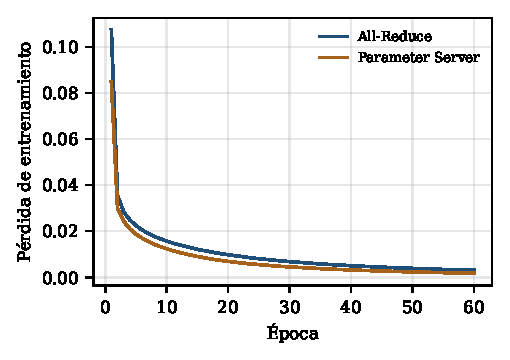
\includegraphics[width=\columnwidth]{mnist_loss_vs_epoch.pdf}
  \caption{Convergencia en MNIST (\texttt{nielsen}, 3 nodos). All-Reduce y Parameter
  Server convergen de forma casi id\'entica; PS queda apenas por debajo.}
  \label{fig:loss}
\end{figure}

\subsection{Comparaci\'on justa y tiempo hasta accuracy}
Bajo \emph{batch global fijo} (240, 40 \'epocas) AR y PS convergen a una accuracy
pr\'acticamente igual: $94.7$\,\% ambos a 5 nodos, y $94.75$ frente a $94.69$\,\% a 3
nodos (\cref{tab:main}). El batch global mayor reduce la accuracy respecto de la receta
de referencia, como era de esperar. La diferencia decisiva es el \emph{tiempo}:
\cref{fig:acctime} y los datos de tiempo hasta convergencia muestran que AR alcanza su
accuracy objetivo en torno a \SI{870}{\second}, mientras PS necesita \SI{1136}{\second}
(cerca de $30$\,\% m\'as) y el baseline \SI{274}{\second}. El servidor central de PS
act\'ua como punto de serializaci\'on.

\begin{figure}[t]
  \centering
  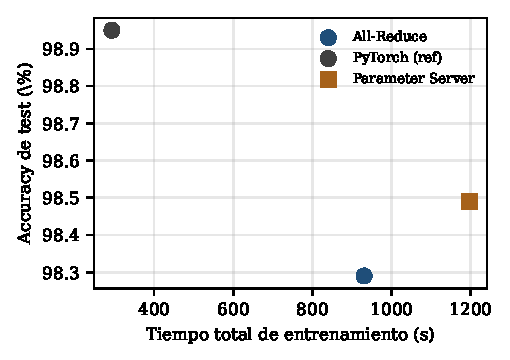
\includegraphics[width=\columnwidth]{mnist_accuracy_vs_time.pdf}
  \caption{Accuracy de test vs.\ tiempo total (MNIST, \texttt{nielsen}, runs de
  referencia). All-Reduce alcanza $\sim$$98.3$\,\% antes que Parameter Server; el
  baseline single-process es el m\'as r\'apido al no pagar comunicaci\'on.}
  \label{fig:acctime}
\end{figure}

\begin{table}[t]\centering
\caption{Resultados principales en MNIST/\texttt{nielsen}.}\label{tab:main}
\footnotesize
\begin{tabular}{lccrrc}\toprule
Estr. & Nodos & Acc.\,(\%) & Tiempo\,(s) & samp./s & Speedup\\\midrule
Baseline & 1 & 98.95 & 294 & 12\,263 & --\\
AR & 3 & 94.75 & 589 & 4\,077 & 1.00\\
PS & 3 & 94.69 & 797 & 3\,012 & 1.00\\
AR & 5 & 94.70 & 493 & 4\,865 & 1.19\\
PS & 5 & 94.75 & 501 & 4\,792 & 1.63\\
\bottomrule\end{tabular}
\end{table}


\subsection{Throughput y escalabilidad}
A batch por worker fijo (64), AR sostiene mayor throughput que PS en ambos tama\~nos
(\cref{fig:throughput}): \SI{4079}{} frente a \SI{2927}{} samples/s a 3 nodos y
\SI{4867}{} frente a \SI{4768}{} a 5. Sin embargo, PS \emph{escala} con pendiente m\'as
pronunciada (\cref{fig:speedup}): al pasar de 3 a 5 nodos su throughput crece
$1.63\times$ (eficiencia $0.81$) contra $1.19\times$ de AR (eficiencia $0.72$), de modo
que casi se igualan a 5 nodos. La lectura: el servidor de PS penaliza el caso chico
pero su costo se amortiza al sumar workers; AR parte m\'as alto pero su anillo
sincr\'onico satura antes los ocho n\'ucleos f\'isicos.

\begin{figure}[t]
  \centering
  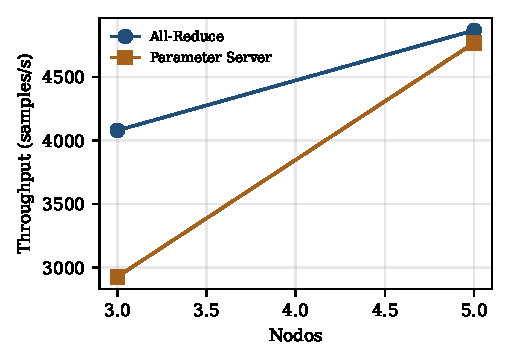
\includegraphics[width=\columnwidth]{throughput_vs_nodes.pdf}
  \caption{Throughput (samples/s) vs.\ nodos, batch por worker fijo. AR domina pero
  PS recorta distancia al crecer los nodos.}
  \label{fig:throughput}
\end{figure}

\begin{figure}[t]
  \centering
  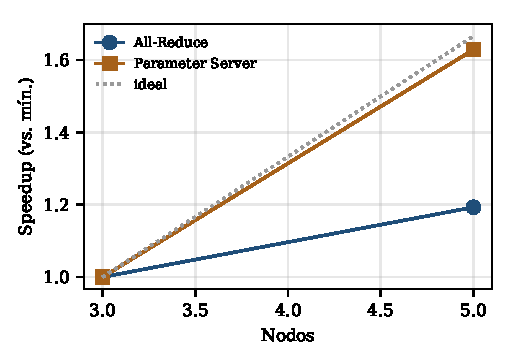
\includegraphics[width=\columnwidth]{speedup_vs_nodes.pdf}
  \caption{Speedup de throughput de 3 a 5 nodos (referencia: la propia config de 3
  nodos). PS escala con mayor pendiente que AR desde una base m\'as baja.}
  \label{fig:speedup}
\end{figure}

\subsection{Presi\'on de comunicaci\'on}
Para aislar el efecto del tama\~no de gradiente entrenamos MLPs de $0.10$, $0.67$ y
$1.86$ millones de par\'ametros (a 3 nodos, batch por worker 64). \Cref{fig:comm} (eje
logar\'itmico) muestra que el throughput se desploma cerca de $40\times$ al crecer el
modelo cerca de $18\times$: la comunicaci\'on, no el c\'omputo, domina. M\'as revelador
es el cruce entre estrategias: con el modelo chico AR aventaja a PS ($\SI{222711}{}$
frente a $\SI{166818}{}$ samples/s, un $34$\,\% m\'as); en el mediano se igualan (PS
incluso arriba, $\SI{25733}{}$ frente a $\SI{23893}{}$); y con el modelo grande AR no
complet\'o el entrenamiento en nuestra configuraci\'on, mientras que PS, con los pesos
shardeados entre servidores, s\'i lo complet\'o ($\SI{5184}{}$ samples/s). Bajo
comunicaci\'on intensa, PS result\'o m\'as robusto. La compresi\'on de gradientes,
esparsa o cuantizada, es una mitigaci\'on conocida para esta
presi\'on~\cite{lin2018deep,aji2017sparse}, fuera del alcance de este trabajo.

\begin{figure}[t]
  \centering
  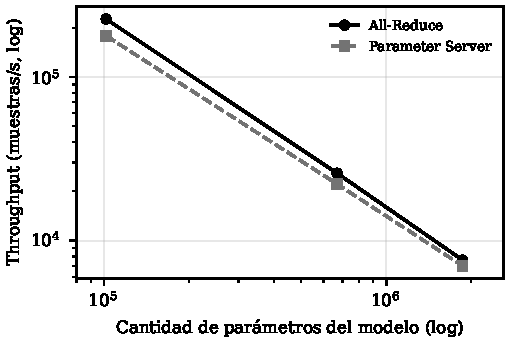
\includegraphics[width=\columnwidth]{communication_pressure.pdf}
  \caption{Presi\'on de comunicaci\'on: throughput (log) vs.\ tama\~no de MLP a 3
  nodos. La ventaja de AR en modelos peque\~nos se diluye al crecer el gradiente; con
  el modelo grande AR no complet\'o el entrenamiento (marca roja) y PS s\'i.}
  \label{fig:comm}
\end{figure}

\section{Discusi\'on}

\textbf{Cu\'ando conviene All-Reduce.} La evidencia favorece AR en el escenario
evaluado: cl\'uster homog\'eneo, red r\'apida (loopback), entrenamiento sincr\'onico y
gradientes densos. Iguala a PS en convergencia y entrega mayor throughput y menor
tiempo hasta accuracy, sin un servidor central que congestione. Es la opci\'on por
defecto cuando no hay heterogeneidad que explotar.

\textbf{Cu\'ando conviene Parameter Server.} Dos evidencias favorecen a PS al crecer la
escala: (i) escala con mayor pendiente al sumar nodos ($1.63\times$ frente a
$1.19\times$), amortizando su costo fijo de servidor; y (ii) bajo comunicaci\'on
intensa fue \emph{m\'as robusto}: con el MLP de $1.86$M de par\'ametros complet\'o el
entrenamiento, donde All-Reduce no lo logr\'o (\cref{fig:comm}). El sharding de pesos
entre servidores reparte la carga de comunicaci\'on. Sus restantes ventajas te\'oricas
(heterogeneidad, stragglers, asincron\'ia) no se ejercitaron y quedan como trabajo
futuro.

\begin{table*}[t]\centering
\caption{Matriz de decisi\'on All-Reduce vs.\ Parameter Server (acotada al entorno evaluado).}\label{tab:decision}
\footnotesize
\begin{tabular}{p{0.30\textwidth}p{0.13\textwidth}p{0.49\textwidth}}\toprule
Condici\'on & Recomendada & Justificaci\'on / evidencia\\\midrule
Cl\'uster homog\'eneo, buena red, sincron\'ia, gradientes densos, evitar servidor central & All-Reduce & Sin punto central de contenci\'on; comunicaci\'on por worker $\approx$ independiente de $W$. \emph{Evidencia:} igual accuracy que PS ($94.7$\,\%) con mayor throughput ($4079$ vs.\ $2927$ samp./s a 3 nodos) y cerca de $30$\,\% menos tiempo hasta accuracy.\\
Modelos grandes, mayor escala, sharding de par\'ametros, desacoplar workers/servers & Parameter Server & El sharding reparte la carga de comunicaci\'on. \emph{Evidencia:} escala con mayor pendiente ($\times1.63$ vs.\ $\times1.19$) y con el MLP de $1.86$M de par\'ametros complet\'o el entrenamiento, donde All-Reduce no lo logr\'o.\\
\bottomrule\end{tabular}
\end{table*}


\subsection{Limitaciones}\label{sec:limits}
El cl\'uster es simulado en una sola m\'aquina de 8 n\'ucleos: el escalado es
l\'ogico, no f\'isico, y la red es loopback (sin latencia ni ancho de banda
realistas). No medimos \emph{test loss} (limitaci\'on del motor) y nos restringimos al
r\'egimen sincr\'onico. No evaluamos stragglers, heterogeneidad de nodos ni datasets
m\'as all\'a de MNIST, que quedan como extensiones reproducibles. O.N.O.\ es un sistema
acad\'emico: \emph{no} compite con frameworks industriales como
Horovod~\cite{sergeev2018horovod} o BytePS~\cite{jiang2020byteps}; los usamos solo como
marco conceptual.

\section{Conclusi\'on}
Respondiendo a la pregunta de investigaci\'on, en el entorno evaluado (homog\'eneo,
sincr\'onico y sobre una sola m\'aquina) \emph{All-Reduce es preferible}: iguala a
Parameter Server en convergencia a batch global fijo y lo supera en throughput y tiempo
hasta accuracy, porque el servidor central de PS introduce un cuello de serializaci\'on.
PS recorta distancia al escalar (mayor pendiente desde una base m\'as baja) y resulta
m\'as robusto con modelos grandes, por lo que ser\'ia la elecci\'on natural si se
explotaran sus ventajas estructurales (heterogeneidad, asincron\'ia, sharding), que
aqu\'i no se ejercitaron. O.N.O.\ aporta evidencia de que un sistema distribuido
implementado desde cero, con asignaci\'on de roles en runtime, permite contrastar ambas
familias bajo un criterio de comparaci\'on justa. Como trabajo futuro: red con latencia
realista, stragglers controlados y la evaluaci\'on de modelos y datasets de mayor
escala.

\bibliographystyle{IEEEtran}
\bibliography{references}

\end{document}
